\chapter{Formulação da cinemática direta}
\label{ch:dir_kin}
%
A cinemática direta permita obter a posição da garra $(x, y, z)$ apartir do ângulo das juntas $(J1, \dots, J6)$. 
Ao contrário da cinemática inversa, a solução existe sempre e é única: para cada conjunto de ângulos há uma, e só uma, posição da garra.

Seguindo a abordagem geométrica da aula, o braço é decomposto em duas partes mais simples: um braço planar, que se move num plano vertical, e uma rotação desse plano em torno do eixo vertical. 
Cada junta tem, por isso, um papel diferente:

\begin{itemize}
    \item A \textbf{junta 1} roda o braço em torno do eixo vertical, logo define a orientação do plano vertical no qual o braço se movimenta;
    \item As \textbf{juntas 2 e 3} comportam-se como um braço planar de 2 DOF, logo é possível aplicar a abordagem geométrica da aula para obter a posição de J4 \textit{(pulso)};
    \item A \textbf{junta 4} define a orientação de $L_4$ e da garra no plano do braço, logo, a partir da posição de J4, permite obter a posição de J5 e do centro de preensão;
    \item A \textbf{junta 5} é fixada a $0^\circ$, para a garra se manter no plano do braço;
    \item A \textbf{junta 6} roda a garra em torno do seu próprio eixo \textit{(yaw)}, logo não afeta a posição do centro de preensão, apenas a direção em que os dedos fecham.
\end{itemize}

A Figura~\ref{fig:3d} mostra o braço numa pose genérica, com os elos, os eixos de rotação de cada junta e a decomposição da posição da garra usada neste capítulo: um desvio lateral $L_5$, uma distância $d$ em frente, no plano do braço, e uma altura $h$.

% Vista 3D do braço
\begin{figure}[H]
  \centering
  \resizebox{0.5\textwidth}{!}{\begin{tikzpicture}[x={(0.10cm,-0.11cm)}, y={(0.26cm,0.04cm)}, z={(0.00cm,0.25cm)}, >=stealth,
                    link/.style={line width=2.4pt, line cap=round, join=round},
                    sombra/.style={line width=2.4pt, line cap=round, gray!30},
                    eixo/.style={->, thin, red!70!black},
                    cota3/.style={dashed, thick, blue!60!black},
                    junta/.style={circle, fill=blue!50, draw=blue!40!black, inner sep=2.2pt}]
  % Coordenadas
    \coordinate (J1) at (0.0,0.0,0.0);
    \coordinate (J2) at (0.0,0.0,13.2);
    \coordinate (J3) at (-1.9,3.3,23.5);
    \coordinate (O) at (3.7,6.5,23.5);
    \coordinate (J4) at (-1.0,14.7,21.9);
    \coordinate (J5) at (-4.7,21.0,21.9);
    \coordinate (J6) at (-4.7,21.0,17.3);
    \coordinate (G) at (-4.7,21.0,6.7);

  % Eixos
    \fill[gray!8] (-12,-6,0) -- (14,-6,0) -- (14,30,0) -- (-12,30,0) -- cycle;
    \draw[->] (0,0,0) -- (14,0,0) node[below] {$x$};
    \draw[->] (0,0,0) -- (0,30,0) node[right] {$y$};
    \draw[->] (0,0,0) -- (0,0,34) node[above] {$z$};

  % Projeção
   \draw[sombra] (0.0,0.0,0) -- (0.0,0.0,0) -- (-1.9,3.3,0) -- (3.7,6.5,0) -- (-1.0,14.7,0) -- (-4.7,21.0,0) -- (-4.7,21.0,0) -- (-4.7,21.0,0);
  
  % Base
    \fill[gray!35] plot[domain=0:360, samples=48, variable=\t] ({4*cos(\t)},{4*sin(\t)},0);
    \fill[gray!25] plot[domain=0:360, samples=48, variable=\t] ({4*cos(\t)},{4*sin(\t)},3);
    \draw[gray!60!black] plot[domain=0:360, samples=48, variable=\t] ({4*cos(\t)},{4*sin(\t)},3);
    \draw[gray!60!black] (1.4,3.8,0) -- (1.4,3.8,3);
    \draw[gray!60!black] (-1.4,-3.8,0) -- (-1.4,-3.8,3);
  
  % Braços
    \draw[link] (J1) -- node[left] {$L_1$} (J2);
    \draw[link] (J2) -- node[left] {$L_2$} (J3);
    \draw[link] (O) -- node[above] {$L_3$} (J4);
    \draw[link] (J4) -- node[above left] {$L_4$} (J5);
    \draw[link] (J5) -- node[right] {$L_6$} (J6);
    \coordinate (palma) at (-4.7,21.0,9.3);
    \draw[link] (J6) -- node[right] {$L_7$} (palma);
 
  % Garra
    \draw[line width=2pt, line cap=round] (-5.7,22.8,9.3) -- (-3.7,19.3,9.3);
    \draw[line width=2pt, line cap=round] (-5.6,22.6,9.3) -- (-5.6,22.6,5.5);
    \draw[line width=2pt, line cap=round] (-3.8,19.5,9.3) -- (-3.8,19.5,5.5);
  
  % Desvio lateral L5 (ao longo do eixo de J3)
    \draw[line width=2.4pt, line cap=round, orange!85!black] (J3) -- (O);
    \draw[thin, gray] (J3) -- (-1.9,3.3,29.0) (O) -- (3.7,6.5,29.0);
    \draw[<->, thin] (-1.9,3.3,28.7) -- node[above=7pt, align=center, font=\small] {$L_5$\\desvio lateral} (3.7,6.5,28.7);
  
  % Cotas
    \coordinate (S) at (5.6,3.2,0.0);
    \coordinate (F) at (-4.7,21.0,0.0);
    \draw[cota3] (0,0,0) -- node[pos=0.6, below=1pt] {$L_5$} (S);
    \draw[cota3] (S) -- node[below=2pt] {$d$} (F);
    \draw[cota3] (F) -- node[pos=0.5, right=2pt] {$h$} (G);
    \draw[blue!60!black, thin] (4.9,4.4,0.0) -- (3.8,3.7,0.0) -- (4.5,2.6,0.0);
    \draw[blue!60!black, thin] (-4.7,21.0,1.3) -- (-4.0,19.9,1.3) -- (-4.0,19.9,0.0);
  
  % Eixos de rotação das juntas
    \draw[eixo] (0.0,0.0,-2.8) -- (0.0,0.0,3.2);
    \draw[eixo] (-2.4,-1.4,13.2) -- (2.8,1.6,13.2);
    \draw[eixo] (-6.2,0.8,23.5) -- (3.2,6.2,23.5);
    \draw[eixo] (-3.4,13.3,21.9) -- (1.8,16.3,21.9);
    \draw[eixo] (-3.3,18.6,21.9) -- (-6.3,23.8,21.9);
    \draw[eixo] (-4.7,21.0,20.1) -- (-4.7,21.0,14.1);
  
  % Juntas
    \node[junta] at (J1) {};
    \node[junta] at (J2) {};
    \node[junta] at (J3) {};
    \node[junta] at (J4) {};
    \node[junta] at (J5) {};
    \node[junta] at (J6) {};
    \node[right=6pt] at (J1) {J1 (base)};
    \node[left=6pt] at (J2) {J2 (ombro)};
    \node[below left=2pt and 4pt] at (J3) {J3 (cotovelo)};
    \node[below=7pt] at (J4) {J4 (pulso)};
    \node[right=7pt] at (J5) {J5};
    \node[right=6pt] at (J6) {J6};
    \fill (G) circle (1.5pt);
    \node[right=12pt, font=\small] at (G) {centro de preensão};
    \draw[eixo] ([shift={(-4.6cm,-0.2cm)}]current bounding box.north east) -- ++(0.7cm,0) node[right, black] {\small eixo de rotação da junta};

  \end{tikzpicture}}
  \caption{Vista 3D do braço.}
  \label{fig:3d}
\end{figure}

O cálculo faz-se em dois passos. Primeiro, no plano lateral, obtêm-se $(d, h)$ a partir de $q_2$, $q_3$ e $q_4$ (Secção~\ref{sec:plano_lateral}). Depois, no plano horizontal, a rotação $q_1$ leva esse ponto para as coordenadas $(x, y, z)$ da base (Secção~\ref{sec:plano_horizontal}).
 
\begin{table}[H]
  \centering
  \caption{Comprimentos dos elos, medidos no cenário do CoppeliaSim.}
  \label{tab:elos}
  \begin{tabular}{llc}
    \hline
    Símbolo & Ligação & Comprimento [m] \\
    \hline
    $L_1$ & base $\rightarrow$ J2 (altura do ombro) & 0,1316 \\
    $L_2$ & J2 $\rightarrow$ J3 & 0,1104 \\
    $L_3$ & J3 $\rightarrow$ J4 & 0,0960 \\
    $L_4$ & J4 $\rightarrow$ J5 & 0,0731 \\
    $L_5$ & desvio lateral J3 $\rightarrow$ J4 & 0,0646 \\
    $L_6$ & J5 $\rightarrow$ J6 & 0,0456 \\
    $L_7$ & J6 $\rightarrow$ centro de preensão & 0,1057 \\
    \hline
  \end{tabular}
\end{table}

% Secções do capítulo
\section{Plano lateral}
\label{sec:plano_lateral}

No plano do braço, como é possível observar na Figura~\ref{fig:lateral}, a posição da garra exprime-se em dois eixos: $d$, a distância em frente, e $h$, a altura acima da base. Neste plano, J2, J3 e J4 têm eixos de rotação paralelos entre si, perpendiculares ao plano, e por isso o braço comporta-se como o braço planar estudado na aula.

\begin{figure}[h]
  \centering
  \resizebox{0.6\textwidth}{!}{%Vista lateral do robô
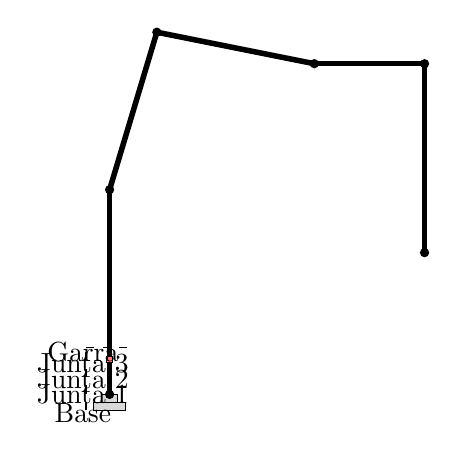
\begin{tikzpicture}[scale=0.2,
                    % Estilos
                    link/.style={line width=2pt, line cap=round},
                    junta/.style={circle, draw, fill=blue!50, line width=1pt, inner sep=2pt}]

  % Coordenadas das juntas
    \coordinate (J1) at (1,1);
    \coordinate (J2) at (1,14);
    \coordinate (J3) at (4,24);
    \coordinate (J4) at (14,22);
    \coordinate (J5) at (21,22);
    \coordinate (J6) at (21,10);

  % Base
    \draw[fill=gray!30] (0,0) rectangle (2,0.5);
    \draw[fill=gray!30] (0.5,0.5) rectangle (1.5,1);
  
  % Juntas
    \draw[junta] (J1) circle (0.2);
    \draw[junta] (J2) circle (0.2);
    \draw[junta] (J3) circle (0.2);
    \draw[junta] (J4) circle (0.2);
    \draw[junta] (J5) circle (0.2);
    \draw[junta] (J6) circle (0.2);
  
  % Braços
    \draw[link] (J1) -- (J2);
    \draw[link] (J2) -- (J3);
    \draw[link] (J3) -- (J4);
    \draw[link] (J4) -- (J5);
    \draw[link] (J5) -- (J6);
  
  % Garra
  \draw[fill=red!50] (0.8,3) rectangle (1.2,3.4);
  
  % Eixos
  \draw[dashed] (-0.5,0) -- (-0.5,4);
  \draw[dashed] (-0.5,4) -- (2.5,4);
  
  % Labels
  \node at (-0.7,-0.2) {Base};
  \node at (-0.7,1) {Junta 1};
  \node at (-0.7,2) {Junta 2};
  \node at (-0.7,3) {Junta 3};
  \node at (-0.7,3.7) {Garra};
\end{tikzpicture}}
  \caption{Vista lateral do braço no seu plano vertical.}
  \label{fig:lateral}
\end{figure}

\subsection{Ângulos absolutos}

Os ângulos das juntas $q_i$ são \underline{relativos}: cada um mede a rotação de um elo em relação ao elo anterior, com o sentido anti-horário positivo. Para somar as projeções de cada elo é mais simples usar ângulos \underline{absolutos}, medidos a partir da horizontal. Como no exemplo do braço de 3 DOF da aula, o ângulo absoluto de cada elo é a soma dos ângulos das juntas anteriores.

Na pose zero (todas as juntas a $0^\circ$) o braço está na vertical, por isso o primeiro elo faz $90^\circ$ com a horizontal quando $q_2 = 0$. A garra é perpendicular ao elo $L_4$. Daqui resultam:
\begin{equation}
    \theta_A = q_2 + \frac{\pi}{2}, \qquad
    \theta_B = \theta_A + q_3, \qquad
    \theta_C = \theta_B + q_4, \qquad
    \alpha = \theta_C - \frac{\pi}{2}
    \label{eq:angulos}
\end{equation}
onde $\theta_A$, $\theta_B$ e $\theta_C$ são os ângulos de $L_2$, $L_3$ e $L_4$ com a horizontal, e $\alpha$ é o ângulo da garra. Com $\alpha = -90^\circ$ a garra aponta na vertical para baixo.

\subsection{Posição de cada junta}

Partindo da base e somando, elo a elo, a projeção horizontal ($L\cos\theta$) e vertical ($L\sin\theta$) de cada elo, obtém-se a posição de cada junta no plano do braço:
\begin{align}
    \text{J2 (ombro):}   \quad & (d_2,\, h_2) = (0,\; L_1) \label{eq:j2}\\
    \text{J3 (cotovelo):} \quad & (d_3,\, h_3) = (d_2 + L_2\cos\theta_A,\; h_2 + L_2\sin\theta_A) \label{eq:j3}\\
    \text{J4 (pulso):}   \quad & (d_4,\, h_4) = (d_3 + L_3\cos\theta_B,\; h_3 + L_3\sin\theta_B) \label{eq:j4}\\
    \text{J5:}           \quad & (d_5,\, h_5) = (d_4 + L_4\cos\theta_C,\; h_4 + L_4\sin\theta_C) \label{eq:j5}
\end{align}

As Equações~\eqref{eq:j3} e~\eqref{eq:j4} são exatamente o braço planar de 2 DOF da aula, com $L_A = L_2$, $L_B = L_3$, $\theta_1 = \theta_A$ e $\theta_2 = q_3$:
\begin{equation}
    x_2 = L_A\cos\theta_1 + L_B\cos(\theta_1 + \theta_2), \qquad
    y_2 = L_A\sin\theta_1 + L_B\sin(\theta_1 + \theta_2)
    \label{eq:2dof}
\end{equation}
com a origem deslocada para o ombro, à altura $L_1$.

\subsection{Posição do centro de preensão}

O centro de preensão está a uma distância $D = L_6 + L_7$ de J5, ao longo da garra, ou seja, na direção $\alpha$. Somando esta última parcela às anteriores, a posição da garra no plano do braço é:
\begin{align}
    d &= L_2\cos\theta_A + L_3\cos\theta_B + L_4\cos\theta_C + D\cos\alpha \label{eq:d}\\
    h &= L_1 + L_2\sin\theta_A + L_3\sin\theta_B + L_4\sin\theta_C + D\sin\alpha \label{eq:h}
\end{align}

Estas equações têm a mesma forma que o braço de 3 DOF da aula ($x_e = L_A\cos\theta_1 + L_B\cos(\theta_1+\theta_2) + L_C\cos(\theta_1+\theta_2+\theta_3)$), com duas diferenças próprias do myCobot: a altura $L_1$ do ombro e o último elo em L, formado por $L_4$ e pela garra $D$, que fazem $90^\circ$ entre si.

\begin{figure}[H]
  \centering
  \resizebox{0.75\textwidth}{!}{\begin{tikzpicture}[scale=0.3, >=stealth,
    elo/.style={line width=2.2pt, line cap=round},
    junta/.style={circle, draw, fill=white, line width=1pt, inner sep=2pt},
    guia/.style={gray!60, thin, densely dotted},
    seg/.style={line width=2.4pt},
    every node/.style={font=\footnotesize}]
  \colorlet{cL1}{gray!70!black}
  \colorlet{cL2}{blue!70!black}
  \colorlet{cL3}{orange!85!black}
  \colorlet{cL4}{green!50!black}
  \colorlet{cD}{violet!80!black}

  % Coordenadas
  \coordinate (B)  at (0,0);
  \coordinate (J2) at (0,13.2);
  \coordinate (J3) at (4.7,23.2);
  \coordinate (J4) at (14.1,21.5);
  \coordinate (J5) at (21.0,24.0);
  \coordinate (G)  at (26.2,9.8);

  % Eixos
  \draw[->, thin] (-2,0) -- (36,0) node[below left] {$d$};
  \draw[->, thin] (B) -- (0,28) node[left] {$h$};
  \fill[gray!25] (-2.5,-0.8) rectangle (2.5,0);

  % Guias
  \foreach \P in {J3,J4,J5,G} \draw[guia] (\P) -- (\P |- 0,-2.2);
  \draw[guia] (J2) -- (29,13.2);
  \draw[guia] (J3) -- (30,23.2);
  \draw[guia] (J4) -- (31,21.5);
  \draw[guia] (J5) -- (32,24.0);
  \draw[guia] (G)  -- (33,9.8);

  % Braços
  \draw[elo, cL1] (B)  -- (J2);
  \draw[elo, cL2] (J2) -- node[left]  {$L_2$} (J3);
  \draw[elo, cL3] (J3) -- node[pos=0.55, above] {$L_3$} (J4);
  \draw[elo, cL4] (J4) -- node[above left] {$L_4$} (J5);
  \draw[elo, cD]  (J5) -- node[right] {$D$} (G);
  \foreach \P in {J2,J3,J4,J5} \node[junta] at (\P) {};
  \fill (G) circle (6pt);
  \node[left=4pt]  at (J2) {J2};
  \node[above=3pt] at (J3) {J3};
  \node[below=4pt] at (J4) {J4};
  \node[above=3pt] at (J5) {J5};
  \node[below left=2pt] at (G) {garra};

  % Ângulos
  \draw[guia] (J2) -- ++(3.5,0);  \draw[->, thin, cL2] ($(J2)+(2.5,0)$) arc[start angle=0, end angle=65, radius=2.5] node[pos=0.4, right] {$\theta_A$};
  \draw[guia] (J3) -- ++(3.5,0);  \draw[->, thin, cL3] ($(J3)+(2.8,0)$) arc[start angle=0, end angle=-10, radius=2.8] node[pos=1, below right=-1pt] {$\theta_B$};
  \draw[guia] (J4) -- ++(3.5,0);  \draw[->, thin, cL4] ($(J4)+(2.8,0)$) arc[start angle=0, end angle=20, radius=2.8] node[pos=0.6, right] {$\theta_C$};
  \draw[guia] (J5) -- ++(3.5,0);  \draw[->, thin, cD]  ($(J5)+(2.5,0)$) arc[start angle=0, end angle=-70, radius=2.5] node[pos=0.6, right] {$\alpha$};

  % Soma de d
  \draw[seg, cL2] (0,-2.2)    -- (4.7,-2.2);
  \draw[seg, cL3] (4.7,-2.2)  -- (14.1,-2.2);
  \draw[seg, cL4] (14.1,-2.2) -- (21.0,-2.2);
  \draw[seg, cD]  (21.0,-2.2) -- (26.2,-2.2);
  \node[cL2, below=3pt] at (2.35,-2.2)  {$L_2\cos\theta_A$};
  \node[cL3, above=3pt] at (9.4,-2.2)   {$L_3\cos\theta_B$};
  \node[cL4, below=3pt] at (17.55,-2.2) {$L_4\cos\theta_C$};
  \node[cD,  above=3pt] at (23.6,-2.2)  {$D\cos\alpha$};
  \draw[|<->|, thin] (0,-5.2) -- node[fill=white, inner sep=1pt] {$d$} (26.2,-5.2);

  % Soma de h
  \draw[seg, cL1, ->] (29,0)    -- (29,13.2);
  \draw[seg, cL2, ->] (30,13.2) -- (30,23.2);
  \draw[seg, cL3, ->] (31,23.2) -- (31,21.5);
  \draw[seg, cL4, ->] (32,21.5) -- (32,24.0);
  \draw[seg, cD,  ->] (33,24.0) -- (33,9.8);
  \draw[guia] (29,13.2) -- (30,13.2) (30,23.2) -- (31,23.2) (31,21.5) -- (32,21.5) (32,24.0) -- (33,24.0);
  \node[cL1, left=1pt]  at (29,6.6)   {$L_1$};
  \node[cL2, right=1pt] at (30,17.5)  {$L_2\sin\theta_A$};
  \node[cL3, right=1pt] at (33.2,22.4) {$L_3\sin\theta_B < 0$};
  \node[cL4, right=1pt] at (32,25.6)  {$L_4\sin\theta_C$};
  \node[cD,  right=1pt] at (33,15.0)  {$D\sin\alpha < 0$};
  \draw[|<->|, thin] (36,0) -- node[fill=white, inner sep=1pt] {$h$} (36,9.8);
  \draw[guia] (33,9.8) -- (36,9.8);
  
\end{tikzpicture}}
  \caption{Somas das projeções dos elos do braço.}
  \label{fig:soma_projecoes}
\end{figure}

\subsection{Juntas 5 e 6}

A junta 5 roda a garra em torno do eixo de $L_4$, tirando-a do plano do braço. Para $q_5 \neq 0$, só a componente $D\cos q_5$ fica no plano e a componente $D\sin q_5$ passa a ser um desvio lateral; as Equações~\eqref{eq:d} e~\eqref{eq:h} ficam
\begin{equation}
    d = \dots + D\cos q_5\cos\alpha, \qquad
    h = \dots + D\cos q_5\sin\alpha, \qquad
    l = L_5 - D\sin q_5
    \label{eq:q5}
\end{equation}
onde $l$ é o desvio lateral total do plano do braço. Como no projeto $q_5 = 0$, tem-se $l = L_5$. A junta 6 roda a garra em torno do seu próprio eixo e não entra nas equações da posição.

\clearpage
\section{\textit{Plano horizontal}}
\label{sec:plano_horizontal}

Numa vista superior do braço, como é possível observar na Figura~\ref{fig:topo}, a \underline{junta 1} é a única junta que roda o plano do braço em torno do eixo vertical. 
As juntas 2, 3 e 4 não mudam a direção desse plano: mudam apenas a distância $d$ em frente e a altura $h$, calculadas na Secção~\ref{sec:plano_lateral}.

\begin{figure}[h]
  \centering
  \resizebox{0.6\textwidth}{!}{%Vista de cima do robô
\begin{tikzpicture}[scale=0.3,
                    % Estilos
                    link/.style={line width=2pt, line cap=round},
                    cota/.style={gray!70!black, thin}]

  % Coordenadas das juntas
    \coordinate (J1) at (0,0);
    \coordinate (J6) at (-4.7,21);     % centro de preensão (x, y)
    \coordinate (O5) at (5.6,3.2);

  % Base
    \draw[->] (-10,0) -- (12,0) node[below left] {$x$};
    \draw[->] (0,-3) -- (0,25) node[left] {$y$};
    \fill[gray!25] (0,0) circle (2.5);  \draw (0,0) circle (2.5);
    \node[below left] at (-2.2,-0.2) {J1};
  
  % Desvio lateral L5 e plano do braço
    \draw[link] (J1) -- node[pos=0.55, below right=-2pt] {$L_5$} (O5);
    \draw[link] (O5) -- node[pos=0.4, right=2pt] {$d$} (J6);
    \draw[cota, dashed] (O5) -- ($(O5)!1.1!(J6)$) node[above, black] {plano do braço};
    \draw[cota, dashed] (O5) -- (30:14);
    \fill (J6) circle (7pt); \node[left=4pt] at (J6) {$(x, y)$};
  
  % Distância
    \draw[cota, dashed] (J1) -- node[pos=0.8, left=1pt, black] {$r$} (J6);
  
  % Ângulos
    \draw[->, thick] (5,0) arc[start angle=0, end angle=30, radius=5] node[pos=0, below right=2pt and -3pt] {$q_1 > 0$};
    \draw[->, thin] (8.5,0) arc[start angle=0, end angle=102.6, radius=8.5] node[pos=0.27, right=2pt] {$\operatorname{atan2}(y, x)$};
    \draw[->, thin] (30:12) arc[start angle=30, end angle=102.6, radius=12] node[pos=0.3, above right=0pt] {$\operatorname{atan2}(d, L_5)$};
    \draw[thin] ($(O5)+(120:1.3)$) -- ($(O5)+(120:1.3)+(210:1.3)$) -- ($(O5)+(210:1.3)$);

  % Convenção de sinal (visto de cima)
    \draw[->, thick, red!70!black] (9,23) ++(-30:1.6) arc[start angle=-30, end angle=250, radius=1.6];
    \node[red!70!black] at (9,23) {$+$};
    \node[right=2pt, align=left, font=\small] at (10.8,23) {ângulo positivo:\\sentido anti-horário};

\end{tikzpicture}}
  \caption{Vista superior do braço no seu plano horizontal.}
  \label{fig:topo}
\end{figure}

\subsection{Desvio lateral}

No MyCobot280, o braço possui um desvio lateral $L_5$ de aproximadamente 6,5 cm, que causa que o plano do braço não intercate o eixo de rotação da junta 1.
O desvio lateral é representado na Figura~\ref{fig:topo} como a distância entre a projeção da junta 3 no plano horizontal e o eixo de rotação da junta 1. 
O desvio lateral é um fator importante a ser considerado no cálculo da cinemática direta, pois ele afeta a posição final da garra no espaço tridimensional.

\subsection{Rotação da base}

Com $q_1 = 0$ a frente do braço aponta para $+y$ e o desvio $L_5$ fica em $+x$. Ao rodar a base de $q_1$ roda-se estas duas direções em torno de $z$, e basta projetar cada parcela nos eixos $x$ e $y$:
 
\begin{itemize}
    \item o desvio lateral $l \ (=L_5)$ faz um ângulo $q_1$ com o eixo $x$, logo contribui com \underline{$l\cos q_1$} em $x$ e \underline{$l\sin q_1$} em $y$;
    \item a distância $d$ em frente é perpendicular ao desvio, ou seja, faz um ângulo $q_1 + 90^\circ$ com o eixo $x$, logo contribui com \underline{$d\cos(q_1 + 90^\circ) = -d\sin q_1$} em $x$ e \underline{$d\sin(q_1 + 90^\circ) = d\cos q_1$} em $y$.
\end{itemize}
 
Somando as duas parcelas, e juntando a altura $h$ do plano lateral:
\begin{equation}
    x = l\cos q_1 - d\sin q_1, \qquad
    y = l\sin q_1 + d\cos q_1, \qquad
    z = h
    \label{eq:xyz}
\end{equation}
 
Sem desvio lateral ($l = 0$), a Equação~\eqref{eq:xyz} reduz-se à forma, $x = d\cos(q_1 + 90^\circ)$ e $y = d\sin(q_1 + 90^\circ)$: a distância ao eixo multiplicada pelo cosseno e pelo seno do ângulo da base.

\subsection{Distância ao eixo da base}

Por o desvio $L_5$ ser perpendicular a $d$, a distância $r$ da garra ao eixo de J1, vista de cima, é
\begin{equation}
    r = \sqrt{x^2 + y^2} = \sqrt{l^2 + d^2}
    \label{eq:r}
\end{equation}
e a direção da garra é $\operatorname{atan2}(y, x) = q_1 + \operatorname{atan2}(d, l)$, como se vê na Figura~\ref{fig:topo}. Esta relação é a usada, ao contrário, na cinemática inversa para obter $q_1$.
 

\clearpage
\section{Resumo e verificação}
\label{sec:dk_resumo}

Juntando os dois planos, a cinemática direta do myCobot 280, com $D = L_6 + L_7$ e os ângulos absolutos da Equação~\eqref{eq:angulos}, é:

\begin{equation}
    \boxed{
    \begin{aligned}
        d &= L_2\cos\theta_A + L_3\cos\theta_B + L_4\cos\theta_C + D\cos q_5\cos\alpha\\
        h &= L_1 + L_2\sin\theta_A + L_3\sin\theta_B + L_4\sin\theta_C + D\cos q_5\sin\alpha\\
        l &= L_5 - D\sin q_5\\[4pt]
        x &= l\cos q_1 - d\sin q_1, \qquad y = l\sin q_1 + d\cos q_1, \qquad z = h
    \end{aligned}}
    \label{eq:dk_final}
\end{equation}

A direção para onde a garra aponta obtém-se da mesma forma, sem os comprimentos: $-\sin q_5$ para o lado, $\cos q_5\cos\alpha$ em frente e $\cos q_5\sin\alpha$ para cima.

Para verificar as equações, a posição dada pela Equação~\eqref{eq:dk_final}, com os ângulos lidos das juntas no simulador, foi comparada com a posição real do centro de preensão no CoppeliaSim: a diferença ficou entre 1,2 e 4,0~mm. Verificou-se também que, aplicando a cinemática inversa a um ponto e a cinemática direta ao resultado, se volta ao mesmo ponto.

\clearpage
